\documentclass[10pt]{article}
\usepackage[T1]{fontenc}
\usepackage[utf8]{inputenc}
\usepackage[default]{sourcesanspro}
\usepackage[letterpaper,left=0.65in,right=0.65in,top=0.75in,bottom=0.75in,headheight=14pt,headsep=10pt,footskip=24pt]{geometry}
\usepackage{fancyhdr}
\usepackage{amssymb}
\usepackage{array,tabularx,xltabular}
\usepackage{enumitem}
\usepackage{needspace}
\usepackage{titlesec}
\usepackage{xcolor}
\usepackage{tikz}

\pagestyle{fancy}
\fancyhf{}
\fancyhead[L]{Week 10 / Bridges / Adult guide}
\fancyfoot[L]{Bellingham Math Circle / Week 10 / F10-FAC-v4}
\fancyfoot[R]{\thepage}
\renewcommand{\headrulewidth}{0.4pt}
\renewcommand{\footrulewidth}{0pt}

\setlength{\parindent}{0pt}
\setlength{\parskip}{4pt}
\raggedright
\frenchspacing
\hyphenpenalty=10000
\exhyphenpenalty=10000

\titleformat{\section}{\large\bfseries}{\thesection.}{0.5em}{}
\titlespacing*{\section}{0pt}{10pt}{3pt}
\titleformat{\subsection}{\normalsize\bfseries}{}{0em}{}
\titlespacing*{\subsection}{0pt}{8pt}{2pt}

\setlist{nosep,leftmargin=1.3em}
\setlist[enumerate]{nosep,leftmargin=1.5em}

\newcolumntype{L}[1]{>{\raggedright\arraybackslash}p{#1}}
\newcolumntype{Y}{>{\raggedright\arraybackslash}X}
\renewcommand{\arraystretch}{1.15}

\tikzset{
  thband/.style={line width=3pt, draw=black!38, line cap=butt},
  thbold/.style={line width=3.4pt, draw=black, line cap=butt},
  thnew/.style={line width=1.4pt, draw=black, dash pattern=on 3pt off 2pt},
  thisland/.style={fill=white, draw=black, line width=0.6pt},
  thfill/.style={fill=black, draw=black, line width=0.6pt},
  thstroke/.style={line width=0.8pt, draw=black!75, line cap=round, line join=round},
  thcross/.style={line width=1.5pt, draw=black},
}

% a K-1 problem block: number and pages, core or not, what the children do
\newcommand{\kprob}[3]{\par\needspace{14\baselineskip}\vspace{3pt}\noindent\textbf{#1}\enspace\textit{#2}\enspace #3\par}
\newcommand{\hints}[1]{\noindent\textbf{Hints:} #1\par}
\newcommand{\ck}{\checkmark}

\begin{document}

{\Large\bfseries Bridges and one-stroke drawings: adult guide}

\section{The idea of the week}

A town is islands joined by bridges. At the start a counter sits on every bridge, and crossing a bridge means picking up its counter, so no bridge can be crossed twice and the counters left show which bridges remain. The question all week: can you pick up every counter, and where do you have to start?

The answer depends only on how many bridges each island has. Each time a walk passes through an island it arrives on one bridge and leaves on another, so it takes that island's counters two at a time. An island with an odd number of bridges (1, 3, 5) must therefore be where the walk starts or ends. So: if no island is odd, you can start anywhere and you end where you started; if exactly two islands are odd, you must start at one and you end at the other; if more are odd, it cannot be done. Tracing a picture without lifting the pencil or going over a line twice is the same question, with corners and crossings as the islands.

The children should find this by walking, getting stuck and noticing which starts worked. Do not tell them the rule; let the counters show them.

What a good session looks like:
\begin{itemize}
\item \textbf{K--1.} Every child walks many towns with the token, puts the counters back and tries again from another island, and says something like ``start where there are three bridges'' or ``this one can't be done, we tried every island''.
\item \textbf{2--3.} Children write walks as letters, count the bridges at each island, state a rule in their own words (Problem 6) and use it on towns they have not walked yet.
\item \textbf{4--5.} Children state the rule and explain why a walk through an island uses its bridges in pairs, settle Königsberg, and the quickest build Lee's walk by joining loops or find the fewest extra counters for a delivery route.
\end{itemize}

\section{Materials and preparation}

\begin{tabularx}{\linewidth}{@{}L{3.6cm}YYYL{2.3cm}@{}}
\hline
 & \textbf{K--1} (4 children, 2 pairs) & \textbf{2--3} (4 children, 2 pairs) & \textbf{4--5} (3 children: pair + referee) & \textbf{Bring in all} \\ \hline
Student packet (12 pages) & 5 copies & 5 copies & 4 copies & 14 packets \\
Counters, about 1 inch or smaller & 20 per pair for the busiest page (page 1, four towns); bag of 50 & 26 per pair for the busiest page (page 7: 22 bridges printed, 4 the children add); bag of 60 & 18 for the busiest page (page 9, Lee's town); bag of 40 so the referee can set up the next town & 150 \\
Tokens unlike the counters (e.g.\ pattern-block triangles): one walks, one marks the start & 2 per pair: 4 & 2 per pair: 4 & 2 & 10 \\
Yellow hexagons & 8 per pair for Problem 7; 20 & 6 per pair for Problem 8; 14 & 6 (for trying ideas) & 40 \\
Craft sticks, 4.5 inch & 12 per pair; 28 & 10 per pair; 24 & 10 & about 60 \\
Coloured pencils & a box to share & a box to share & 4 colours per child (Problem 7) & \\
Pencils, erasers, scrap paper, small whiteboards & 1 each & 1 each & 1 each & \\
Small sticky notes & & 1 pad, to letter hexagons (Problem 8) & 1 pad & 2 pads \\ \hline
\end{tabularx}

Also: masking tape and 6 counters (or sticky notes) for the floor town; 3 copies of this guide.

\textbf{Printing.} Print every page single-sided on Letter paper at 100\% (``actual size''). ``Fit to page'' shrinks the bridges below counter size. Give out one page at a time. A pair walks on one copy; each child records on their own copy. Some problems continue onto the next page: K--1 Problems 3--6 and 8, 2--3 Problems 2--5 and 7, 4--5 Problems 2, 3, 7 and 10. Hand out both pages together. Nothing needs cutting.

\textbf{Floor town (optional, for the launch).} Before the children arrive, tape the house town from page 1 on the floor in open space: 5 islands (tape circles or paper plates about 1 foot across) in the shape of a square with a roof, joined by 6 tape bridges 3--4 feet long. Put a counter or a sticky note in the middle of each bridge.

\textbf{Test with the real materials before the session.}
\begin{enumerate}
\item \textbf{Counters fit.} The bridges are grey bands 1.6\,cm (5/8 inch) wide and at least 3\,cm long, sized for counters about 1 inch across. A 1-inch counter is wider than the band; that is expected. On K--1 page 9, second town (square with a centre island, the tightest town), put a counter in the middle of all 8 bridges. Each should sit on its own band without covering an island or another counter. If yours are bigger, use something smaller: any small token works (buttons, coins, beans).
\item \textbf{Double bridges.} Lay two craft sticks side by side between two hexagons; both should touch both hexagons and hold a counter. 2--3 Problem 8 needs this: its first and last towns cannot be built without two bridges between the same two islands.
\item \textbf{Two counters on one bridge} (K--1 Problem 8, 2--3 Problem 10, 4--5 Problem 10): stack them. Crossing takes the top one. Show it the same way at all tables.
\end{enumerate}

\section{The hour}

\begin{tabularx}{\linewidth}{@{}L{1.6cm}Y@{}}
\hline
0--5 min & Running around. \\
5--8 & Whole-group launch at the floor town (below). \\
8--50 & Tables, in pairs. Fallback activity when attention runs out. \\
50--57 & Sharing: one question for everyone (below). \\
57--60 & Count the counters back into the bags. \\ \hline
\end{tabularx}

\textbf{Launch (organizer, 2--3 minutes).} Everyone stands around the floor town. Without one, hold up K--1 page 1 with counters on the house town and gather the children around one table.
\begin{enumerate}
\item Adult points: ``This is a town. The circles are islands and the tape lines are bridges. Every bridge has a counter on it.''
\item Adult: ``You walk from island to island over the bridges. When you cross a bridge, you pick up its counter. A bridge with no counter is closed: you cannot cross it.''
\item One child stands on a bottom corner island, walks along the bottom bridge, and picks up its counter. That is a legal move.
\item Adult points at the empty bridge: ``Can she go back across this one?'' (No: no counter.) ``Keep going.'' From a bottom corner the child is sure to get stuck with counters left.
\item Adult: ``Counters are left. Would a different start pick up every counter? That is your question today. At your table you will walk towns on paper with counters.'' Do not say which start works.
\end{enumerate}

\textbf{Pairs.}
\begin{itemize}
\item \textbf{K--1}: two pairs, each a kindergartner with a first grader. The walker moves the token and picks up counters. The keeper puts every counter back before each try and says ``stop'' if the token crosses a bridge with no counter. Swap after each town.
\item \textbf{2--3}: two pairs. One walks with the token; the other writes the walk as letters while it happens and keeps the counters. Swap after each town.
\item \textbf{4--5}: one pair works; the third child is referee. The referee checks every move, resets counters, and must try to beat every ``none'' or ``fewest'' answer before it is written down. Rotate the referee at each new problem.
\end{itemize}

\textbf{Fallback when attention runs out.}
\begin{itemize}
\item \textbf{K--1}: each child builds a town with hexagons and sticks, puts a counter on every stick, and the partner tries to pick up every counter. Or walk the floor town.
\item \textbf{2--3 and 4--5}: the bridge game on the house town (Problem 1, first town). Counters on all bridges, one shared token on an island. Players take turns moving the token across one bridge and keeping its counter. A player who cannot move loses. For the adult: starting on B or C, the second player can always win; starting on A, D or E, the first player can. 4--5 can try to work out why, then play on other towns from the packet.
\end{itemize}

\textbf{Sharing question} (each table shows one town): ``Show us a town where nobody can pick up every counter. How do you know nobody can?''

\section{Table by table}

\subsection{K--1 (parent volunteer)}

Read each problem aloud once. Put counters on the bridges of one town at a time and let the pair walk it. Before every new try, all counters go back. Put a small pencil dot on each island you have already tried as a start.

\textbf{Things to say:} ``Where are you stuck? Which counters are left?'' \;``Put them all back. Try another island.'' \;``Did that island work? Let's put a dot on it.'' \;``Count the bridges at this island with your finger.'' Let the counters decide; you do not need to say whether a start is good.

\textbf{Core of the hour:} Problems 1--3. \textbf{Next:} 4 and 5. \textbf{For children who get further:} 6--8. \textbf{If a child is struggling:} one town at a time, you hold the counters bag, skip the big triangle in Problem 2, and switch to Problem 5 (tracing) or Problem 7 (building) before coming back.

In the answer pictures, \textbf{filled islands} are where a walk that picks up every counter can start. The walk then ends on the other filled island. When every island is filled, it ends where it started.

\kprob{Problem 1}{page 1, core}{Pick up every counter in each of four towns; colour the island you started on.}
\par\smallskip\noindent\hfill\begin{tabular}[b]{@{}c@{}}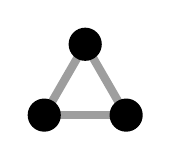
\begin{tikzpicture}
\draw[thband] (0.200,0.200) -- (1.240,0.200);
\draw[thband] (1.240,0.200) -- (0.720,1.100);
\draw[thband] (0.720,1.100) -- (0.200,0.200);
\draw[thfill] (0.200,0.200) circle (0.200);
\draw[thfill] (1.240,0.200) circle (0.200);
\draw[thfill] (0.720,1.100) circle (0.200);
\end{tikzpicture}\\[1pt]\parbox[t]{2.90cm}{\centering\footnotesize start anywhere}\end{tabular}\hfill
\begin{tabular}[b]{@{}c@{}}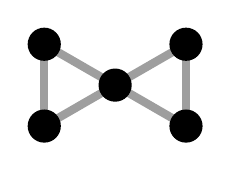
\begin{tikzpicture}
\draw[thband] (1.100,0.720) -- (0.200,1.239);
\draw[thband] (0.200,1.239) -- (0.200,0.200);
\draw[thband] (0.200,0.200) -- (1.100,0.720);
\draw[thband] (1.100,0.720) -- (2.000,1.239);
\draw[thband] (2.000,1.239) -- (2.000,0.200);
\draw[thband] (2.000,0.200) -- (1.100,0.720);
\draw[thfill] (0.200,1.239) circle (0.200);
\draw[thfill] (0.200,0.200) circle (0.200);
\draw[thfill] (1.100,0.720) circle (0.200);
\draw[thfill] (2.000,1.239) circle (0.200);
\draw[thfill] (2.000,0.200) circle (0.200);
\end{tikzpicture}\\[1pt]\parbox[t]{2.90cm}{\centering\footnotesize start anywhere}\end{tabular}\hfill
\begin{tabular}[b]{@{}c@{}}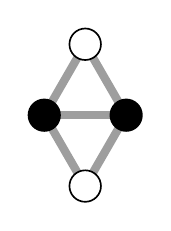
\begin{tikzpicture}
\draw[thband] (0.200,1.100) -- (1.240,1.100);
\draw[thband] (0.200,1.100) -- (0.720,2.001);
\draw[thband] (1.240,1.100) -- (0.720,2.001);
\draw[thband] (0.200,1.100) -- (0.720,0.200);
\draw[thband] (1.240,1.100) -- (0.720,0.200);
\draw[thisland] (0.720,2.001) circle (0.200);
\draw[thfill] (0.200,1.100) circle (0.200);
\draw[thfill] (1.240,1.100) circle (0.200);
\draw[thisland] (0.720,0.200) circle (0.200);
\end{tikzpicture}\\[1pt]\parbox[t]{2.90cm}{\centering\footnotesize start on a filled island}\end{tabular}\hfill
\begin{tabular}[b]{@{}c@{}}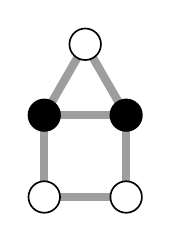
\begin{tikzpicture}
\draw[thband] (0.200,0.200) -- (1.240,0.200);
\draw[thband] (1.240,0.200) -- (1.240,1.239);
\draw[thband] (1.240,1.239) -- (0.200,1.239);
\draw[thband] (0.200,1.239) -- (0.200,0.200);
\draw[thband] (0.200,1.239) -- (0.720,2.140);
\draw[thband] (0.720,2.140) -- (1.240,1.239);
\draw[thisland] (0.200,0.200) circle (0.200);
\draw[thisland] (1.240,0.200) circle (0.200);
\draw[thfill] (1.240,1.239) circle (0.200);
\draw[thfill] (0.200,1.239) circle (0.200);
\draw[thisland] (0.720,2.140) circle (0.200);
\end{tikzpicture}\\[1pt]\parbox[t]{2.90cm}{\centering\footnotesize start on a filled island}\end{tabular}\hfill\null\par\smallskip

\hints{1. ``Put the counters back and start on a different island.'' \;2. ``Count the bridges at each island. Try one that has 3.'' \;3. Point to a filled island.}

\kprob{Problem 2}{page 2, core}{Colour every island where the token can start and still pick up every counter.}
\par\smallskip\noindent\hfill\begin{tabular}[b]{@{}c@{}}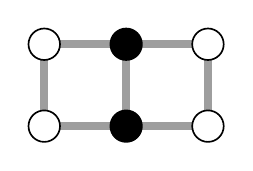
\begin{tikzpicture}
\draw[thband] (0.200,0.200) -- (1.240,0.200);
\draw[thband] (0.200,1.240) -- (1.240,1.240);
\draw[thband] (1.240,0.200) -- (2.279,0.200);
\draw[thband] (1.240,1.240) -- (2.279,1.240);
\draw[thband] (0.200,0.200) -- (0.200,1.240);
\draw[thband] (1.240,0.200) -- (1.240,1.240);
\draw[thband] (2.279,0.200) -- (2.279,1.240);
\draw[thisland] (0.200,0.200) circle (0.200);
\draw[thfill] (1.240,0.200) circle (0.200);
\draw[thisland] (2.279,0.200) circle (0.200);
\draw[thisland] (0.200,1.240) circle (0.200);
\draw[thfill] (1.240,1.240) circle (0.200);
\draw[thisland] (2.279,1.240) circle (0.200);
\end{tikzpicture}\\[1pt]\parbox[t]{2.90cm}{\centering\footnotesize only the 2 filled islands}\end{tabular}\hfill
\begin{tabular}[b]{@{}c@{}}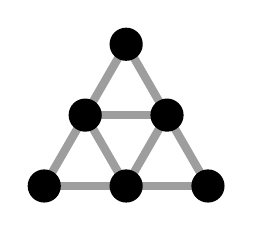
\begin{tikzpicture}
\draw[thband] (0.200,0.200) -- (1.240,0.200);
\draw[thband] (1.240,0.200) -- (2.279,0.200);
\draw[thband] (2.279,0.200) -- (1.759,1.100);
\draw[thband] (1.759,1.100) -- (1.240,2.000);
\draw[thband] (1.240,2.000) -- (0.720,1.100);
\draw[thband] (0.720,1.100) -- (0.200,0.200);
\draw[thband] (1.240,0.200) -- (1.759,1.100);
\draw[thband] (1.759,1.100) -- (0.720,1.100);
\draw[thband] (0.720,1.100) -- (1.240,0.200);
\draw[thfill] (0.200,0.200) circle (0.200);
\draw[thfill] (1.240,0.200) circle (0.200);
\draw[thfill] (2.279,0.200) circle (0.200);
\draw[thfill] (0.720,1.100) circle (0.200);
\draw[thfill] (1.759,1.100) circle (0.200);
\draw[thfill] (1.240,2.000) circle (0.200);
\end{tikzpicture}\\[1pt]\parbox[t]{2.90cm}{\centering\footnotesize every island}\end{tabular}\hfill\null\par\smallskip

Two squares: only the two middle islands (each has 3 bridges); the walk ends on the other one. Big triangle: every island works, and the walk ends where it started. The children must try every island to know they have them all.
\hints{1. ``Let's try every island, one at a time, and put a dot on each one that works.'' \;2. ``What is different about the islands that worked?'' \;3. ``Count the bridges at them, and at the others.''}

\kprob{Problem 3}{pages 3--4, core}{Can you pick up every counter? Check if yes, X if no.}
\par\smallskip\noindent\hfill\begin{tabular}[b]{@{}c@{}}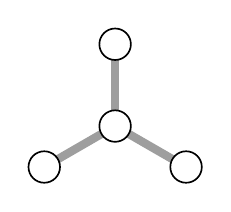
\begin{tikzpicture}
\draw[thband] (1.100,0.720) -- (1.100,1.759);
\draw[thband] (1.100,0.720) -- (0.200,0.200);
\draw[thband] (1.100,0.720) -- (2.001,0.200);
\draw[thisland] (1.100,0.720) circle (0.200);
\draw[thisland] (1.100,1.759) circle (0.200);
\draw[thisland] (0.200,0.200) circle (0.200);
\draw[thisland] (2.001,0.200) circle (0.200);
\end{tikzpicture}\\[1pt]\parbox[t]{2.90cm}{\centering\footnotesize \textbf{X}}\end{tabular}\hfill
\begin{tabular}[b]{@{}c@{}}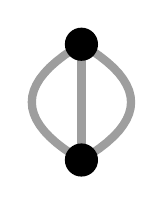
\begin{tikzpicture}
\draw[thband] (0.630,0.200) -- (0.630,1.670);
\draw[thband] (0.630,0.200) -- (0.510,0.274) -- (0.403,0.347) -- (0.309,0.420) -- (0.227,0.494) -- (0.158,0.567) -- (0.101,0.641) -- (0.057,0.714) -- (0.025,0.788) -- (0.006,0.861) -- (0.000,0.935) -- (0.006,1.008) -- (0.025,1.082) -- (0.057,1.155) -- (0.101,1.229) -- (0.158,1.302) -- (0.227,1.376) -- (0.309,1.449) -- (0.403,1.523) -- (0.510,1.597) -- (0.630,1.670) -- (0.630,1.670);
\draw[thband] (0.630,0.200) -- (0.750,0.274) -- (0.857,0.347) -- (0.951,0.420) -- (1.033,0.494) -- (1.103,0.567) -- (1.159,0.641) -- (1.203,0.714) -- (1.235,0.788) -- (1.254,0.861) -- (1.260,0.935) -- (1.254,1.008) -- (1.235,1.082) -- (1.203,1.155) -- (1.159,1.229) -- (1.103,1.302) -- (1.033,1.376) -- (0.951,1.449) -- (0.857,1.523) -- (0.750,1.597) -- (0.630,1.670) -- (0.630,1.670);
\draw[thfill] (0.630,0.200) circle (0.200);
\draw[thfill] (0.630,1.670) circle (0.200);
\end{tikzpicture}\\[1pt]\parbox[t]{2.90cm}{\centering\footnotesize \checkmark\ any island}\end{tabular}\hfill
\begin{tabular}[b]{@{}c@{}}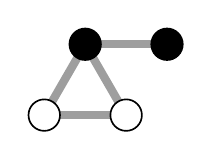
\begin{tikzpicture}
\draw[thband] (0.200,0.200) -- (1.240,0.200);
\draw[thband] (1.240,0.200) -- (0.720,1.100);
\draw[thband] (0.720,1.100) -- (0.200,0.200);
\draw[thband] (0.720,1.100) -- (1.759,1.100);
\draw[thisland] (0.200,0.200) circle (0.200);
\draw[thisland] (1.240,0.200) circle (0.200);
\draw[thfill] (0.720,1.100) circle (0.200);
\draw[thfill] (1.759,1.100) circle (0.200);
\end{tikzpicture}\\[1pt]\parbox[t]{2.90cm}{\centering\footnotesize \checkmark\ start on a filled island}\end{tabular}\hfill
\begin{tabular}[b]{@{}c@{}}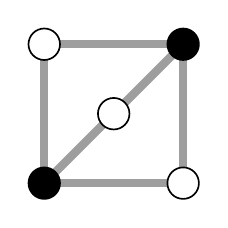
\begin{tikzpicture}
\draw[thband] (0.200,0.200) -- (1.964,0.200);
\draw[thband] (1.964,0.200) -- (1.964,1.964);
\draw[thband] (1.964,1.964) -- (0.200,1.964);
\draw[thband] (0.200,1.964) -- (0.200,0.200);
\draw[thband] (1.082,1.082) -- (0.200,0.200);
\draw[thband] (1.082,1.082) -- (1.964,1.964);
\draw[thfill] (0.200,0.200) circle (0.200);
\draw[thisland] (1.964,0.200) circle (0.200);
\draw[thfill] (1.964,1.964) circle (0.200);
\draw[thisland] (0.200,1.964) circle (0.200);
\draw[thisland] (1.082,1.082) circle (0.200);
\end{tikzpicture}\\[1pt]\parbox[t]{2.90cm}{\centering\footnotesize \checkmark\ start on a filled island}\end{tabular}\hfill
\begin{tabular}[b]{@{}c@{}}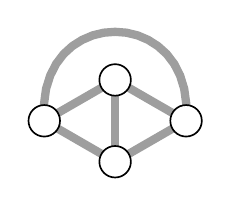
\begin{tikzpicture}
\draw[thband] (1.100,1.239) -- (1.100,0.200);
\draw[thband] (1.100,1.239) -- (0.200,0.720);
\draw[thband] (1.100,1.239) -- (2.001,0.720);
\draw[thband] (1.100,0.200) -- (0.200,0.720);
\draw[thband] (1.100,0.200) -- (2.001,0.720);
\draw[thband] (0.200,0.720) -- (0.197,0.935) -- (0.223,1.127) -- (0.276,1.296) -- (0.351,1.443) -- (0.446,1.568) -- (0.557,1.669) -- (0.682,1.748) -- (0.816,1.805) -- (0.956,1.839) -- (1.100,1.850) -- (1.244,1.839) -- (1.385,1.805) -- (1.519,1.748) -- (1.643,1.669) -- (1.755,1.568) -- (1.850,1.443) -- (1.925,1.296) -- (1.977,1.127) -- (2.004,0.935) -- (2.001,0.720) -- (2.001,0.720);
\draw[thisland] (1.100,1.239) circle (0.200);
\draw[thisland] (1.100,0.200) circle (0.200);
\draw[thisland] (0.200,0.720) circle (0.200);
\draw[thisland] (2.001,0.720) circle (0.200);
\end{tikzpicture}\\[1pt]\parbox[t]{2.90cm}{\centering\footnotesize \textbf{X}}\end{tabular}\hfill\null\par\smallskip

Answers in order: X, \ck, \ck, \ck, X. Why the three-arm star is impossible, in a child's words: ``Each tip has one bridge. If you go onto a tip you can't get off, so a tip can only be where you start or where you finish. There are three tips.'' In the last town every island has 3 bridges, so all four islands have the same trouble.
\hints{1. ``Try two different starts.'' \;2. ``When you go onto a tip, can you get off again?'' \;3. For a \ck\ town, point to a filled island.}

\kprob{Problem 4}{pages 5--6}{Pick up every counter and end on the island where you started. Check or X.}
\par\smallskip\noindent\hfill\begin{tabular}[b]{@{}c@{}}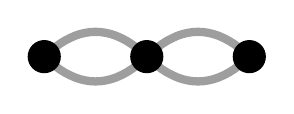
\begin{tikzpicture}
\draw[thband] (0.200,0.315) -- (0.265,0.375) -- (0.330,0.428) -- (0.395,0.476) -- (0.460,0.517) -- (0.526,0.551) -- (0.591,0.580) -- (0.656,0.602) -- (0.721,0.617) -- (0.786,0.627) -- (0.851,0.630) -- (0.916,0.627) -- (0.981,0.617) -- (1.046,0.602) -- (1.111,0.580) -- (1.177,0.551) -- (1.242,0.517) -- (1.307,0.476) -- (1.372,0.428) -- (1.437,0.375) -- (1.502,0.315) -- (1.502,0.315);
\draw[thband] (0.200,0.315) -- (0.265,0.255) -- (0.330,0.202) -- (0.395,0.154) -- (0.460,0.113) -- (0.526,0.079) -- (0.591,0.050) -- (0.656,0.028) -- (0.721,0.013) -- (0.786,0.003) -- (0.851,0.000) -- (0.916,0.003) -- (0.981,0.013) -- (1.046,0.028) -- (1.111,0.050) -- (1.177,0.079) -- (1.242,0.113) -- (1.307,0.154) -- (1.372,0.202) -- (1.437,0.255) -- (1.502,0.315) -- (1.502,0.315);
\draw[thband] (1.502,0.315) -- (1.567,0.375) -- (1.632,0.428) -- (1.697,0.476) -- (1.762,0.517) -- (1.828,0.551) -- (1.893,0.580) -- (1.958,0.602) -- (2.023,0.617) -- (2.088,0.627) -- (2.153,0.630) -- (2.218,0.627) -- (2.283,0.617) -- (2.348,0.602) -- (2.413,0.580) -- (2.479,0.551) -- (2.544,0.517) -- (2.609,0.476) -- (2.674,0.428) -- (2.739,0.375) -- (2.804,0.315) -- (2.804,0.315);
\draw[thband] (1.502,0.315) -- (1.567,0.255) -- (1.632,0.202) -- (1.697,0.154) -- (1.762,0.113) -- (1.828,0.079) -- (1.893,0.050) -- (1.958,0.028) -- (2.023,0.013) -- (2.088,0.003) -- (2.153,0.000) -- (2.218,0.003) -- (2.283,0.013) -- (2.348,0.028) -- (2.413,0.050) -- (2.479,0.079) -- (2.544,0.113) -- (2.609,0.154) -- (2.674,0.202) -- (2.739,0.255) -- (2.804,0.315) -- (2.804,0.315);
\draw[thfill] (0.200,0.315) circle (0.200);
\draw[thfill] (1.502,0.315) circle (0.200);
\draw[thfill] (2.804,0.315) circle (0.200);
\end{tikzpicture}\\[1pt]\parbox[t]{3.10cm}{\centering\footnotesize \checkmark}\end{tabular}\hfill
\begin{tabular}[b]{@{}c@{}}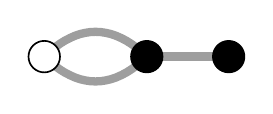
\begin{tikzpicture}
\draw[thband] (0.200,0.315) -- (0.265,0.375) -- (0.330,0.428) -- (0.395,0.476) -- (0.460,0.517) -- (0.526,0.551) -- (0.591,0.580) -- (0.656,0.602) -- (0.721,0.617) -- (0.786,0.627) -- (0.851,0.630) -- (0.916,0.627) -- (0.981,0.617) -- (1.046,0.602) -- (1.111,0.580) -- (1.177,0.551) -- (1.242,0.517) -- (1.307,0.476) -- (1.372,0.428) -- (1.437,0.375) -- (1.502,0.315) -- (1.502,0.315);
\draw[thband] (0.200,0.315) -- (0.265,0.255) -- (0.330,0.202) -- (0.395,0.154) -- (0.460,0.113) -- (0.526,0.079) -- (0.591,0.050) -- (0.656,0.028) -- (0.721,0.013) -- (0.786,0.003) -- (0.851,0.000) -- (0.916,0.003) -- (0.981,0.013) -- (1.046,0.028) -- (1.111,0.050) -- (1.177,0.079) -- (1.242,0.113) -- (1.307,0.154) -- (1.372,0.202) -- (1.437,0.255) -- (1.502,0.315) -- (1.502,0.315);
\draw[thband] (1.502,0.315) -- (2.542,0.315);
\draw[thisland] (0.200,0.315) circle (0.200);
\draw[thfill] (1.502,0.315) circle (0.200);
\draw[thfill] (2.542,0.315) circle (0.200);
\end{tikzpicture}\\[1pt]\parbox[t]{2.90cm}{\centering\footnotesize \textbf{X} (ends elsewhere)}\end{tabular}\hfill
\begin{tabular}[b]{@{}c@{}}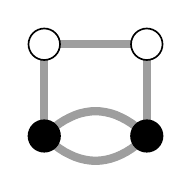
\begin{tikzpicture}
\draw[thband] (0.200,0.315) -- (0.265,0.375) -- (0.330,0.428) -- (0.395,0.476) -- (0.460,0.517) -- (0.526,0.551) -- (0.591,0.580) -- (0.656,0.602) -- (0.721,0.617) -- (0.786,0.627) -- (0.851,0.630) -- (0.916,0.627) -- (0.981,0.617) -- (1.046,0.602) -- (1.111,0.580) -- (1.177,0.551) -- (1.242,0.517) -- (1.307,0.476) -- (1.372,0.428) -- (1.437,0.375) -- (1.502,0.315) -- (1.502,0.315);
\draw[thband] (0.200,0.315) -- (0.265,0.255) -- (0.330,0.202) -- (0.395,0.154) -- (0.460,0.113) -- (0.526,0.079) -- (0.591,0.050) -- (0.656,0.028) -- (0.721,0.013) -- (0.786,0.003) -- (0.851,0.000) -- (0.916,0.003) -- (0.981,0.013) -- (1.046,0.028) -- (1.111,0.050) -- (1.177,0.079) -- (1.242,0.113) -- (1.307,0.154) -- (1.372,0.202) -- (1.437,0.255) -- (1.502,0.315) -- (1.502,0.315);
\draw[thband] (1.502,0.315) -- (1.502,1.480);
\draw[thband] (1.502,1.480) -- (0.200,1.480);
\draw[thband] (0.200,1.480) -- (0.200,0.315);
\draw[thfill] (0.200,0.315) circle (0.200);
\draw[thfill] (1.502,0.315) circle (0.200);
\draw[thisland] (1.502,1.480) circle (0.200);
\draw[thisland] (0.200,1.480) circle (0.200);
\end{tikzpicture}\\[1pt]\parbox[t]{2.90cm}{\centering\footnotesize \textbf{X} (ends elsewhere)}\end{tabular}\hfill
\begin{tabular}[b]{@{}c@{}}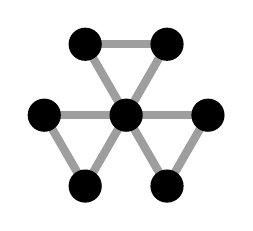
\begin{tikzpicture}
\draw[thband] (1.240,1.100) -- (1.759,2.001);
\draw[thband] (1.759,2.001) -- (0.720,2.001);
\draw[thband] (0.720,2.001) -- (1.240,1.100);
\draw[thband] (1.240,1.100) -- (0.200,1.100);
\draw[thband] (0.200,1.100) -- (0.720,0.200);
\draw[thband] (0.720,0.200) -- (1.240,1.100);
\draw[thband] (1.240,1.100) -- (1.759,0.200);
\draw[thband] (1.759,0.200) -- (2.279,1.100);
\draw[thband] (2.279,1.100) -- (1.240,1.100);
\draw[thfill] (1.240,1.100) circle (0.200);
\draw[thfill] (1.759,2.001) circle (0.200);
\draw[thfill] (0.720,2.001) circle (0.200);
\draw[thfill] (0.200,1.100) circle (0.200);
\draw[thfill] (0.720,0.200) circle (0.200);
\draw[thfill] (1.759,0.200) circle (0.200);
\draw[thfill] (2.279,1.100) circle (0.200);
\end{tikzpicture}\\[1pt]\parbox[t]{2.90cm}{\centering\footnotesize \checkmark}\end{tabular}\hfill
\begin{tabular}[b]{@{}c@{}}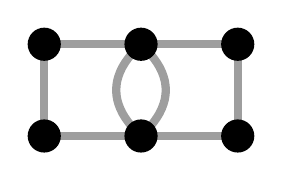
\begin{tikzpicture}
\draw[thband] (0.200,0.200) -- (1.429,0.200);
\draw[thband] (0.200,1.365) -- (1.429,1.365);
\draw[thband] (1.429,0.200) -- (2.657,0.200);
\draw[thband] (1.429,1.365) -- (2.657,1.365);
\draw[thband] (0.200,0.200) -- (0.200,1.365);
\draw[thband] (2.657,0.200) -- (2.657,1.365);
\draw[thband] (1.429,0.200) -- (1.369,0.258) -- (1.315,0.317) -- (1.268,0.375) -- (1.227,0.433) -- (1.192,0.491) -- (1.164,0.550) -- (1.142,0.608) -- (1.126,0.666) -- (1.117,0.724) -- (1.114,0.783) -- (1.117,0.841) -- (1.126,0.899) -- (1.142,0.957) -- (1.164,1.016) -- (1.192,1.074) -- (1.227,1.132) -- (1.268,1.190) -- (1.315,1.249) -- (1.369,1.307) -- (1.429,1.365) -- (1.429,1.365);
\draw[thband] (1.429,0.200) -- (1.488,0.258) -- (1.542,0.317) -- (1.589,0.375) -- (1.630,0.433) -- (1.665,0.491) -- (1.693,0.550) -- (1.715,0.608) -- (1.731,0.666) -- (1.740,0.724) -- (1.744,0.783) -- (1.740,0.841) -- (1.731,0.899) -- (1.715,0.957) -- (1.693,1.016) -- (1.665,1.074) -- (1.630,1.132) -- (1.589,1.190) -- (1.542,1.249) -- (1.488,1.307) -- (1.429,1.365) -- (1.429,1.365);
\draw[thfill] (0.200,0.200) circle (0.200);
\draw[thfill] (0.200,1.365) circle (0.200);
\draw[thfill] (1.429,0.200) circle (0.200);
\draw[thfill] (1.429,1.365) circle (0.200);
\draw[thfill] (2.657,0.200) circle (0.200);
\draw[thfill] (2.657,1.365) circle (0.200);
\end{tikzpicture}\\[1pt]\parbox[t]{2.96cm}{\centering\footnotesize \checkmark}\end{tabular}\hfill\null\par\smallskip

Answers in order: \ck, X, X, \ck, \ck. In the two X towns you can pick up every counter (start on a filled island), but you finish on the other filled island, not back home.
\hints{1. ``Put the extra token on the island where you start, so we remember it.'' \;2. ``Where did you finish? Can you finish on the marked island?'' \;3. ``This island has 3 bridges: out, back, out again. Can you get home?''}

\kprob{Problem 5}{pages 7--8}{Trace each picture with a coloured pencil without lifting it or going over a line twice; cross out the ones that cannot be done. Each picture is printed twice so a child gets a second try.}
\par\smallskip\noindent\hfill\begin{tabular}[b]{@{}c@{}}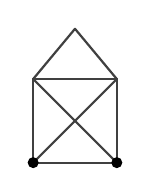
\begin{tikzpicture}
\draw[thstroke] (0.000,0.000) -- (1.062,0.000);
\draw[thstroke] (1.062,0.000) -- (1.062,1.062);
\draw[thstroke] (1.062,1.062) -- (0.000,1.062);
\draw[thstroke] (0.000,1.062) -- (0.000,0.000);
\draw[thstroke] (0.000,0.000) -- (1.062,1.062);
\draw[thstroke] (1.062,0.000) -- (0.000,1.062);
\draw[thstroke] (0.000,1.062) -- (0.531,1.700);
\draw[thstroke] (0.531,1.700) -- (1.062,1.062);
\fill (0.000,0.000) circle (0.07);
\fill (1.062,0.000) circle (0.07);
\end{tikzpicture}\\[1pt]\parbox[t]{2.90cm}{\centering\footnotesize start at a dot}\end{tabular}\hfill
\begin{tabular}[b]{@{}c@{}}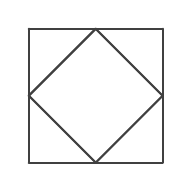
\begin{tikzpicture}
\draw[thstroke] (0.000,0.000) -- (1.700,0.000);
\draw[thstroke] (1.700,0.000) -- (1.700,1.700);
\draw[thstroke] (1.700,1.700) -- (0.000,1.700);
\draw[thstroke] (0.000,1.700) -- (0.000,0.000);
\draw[thstroke] (0.850,0.000) -- (1.700,0.850);
\draw[thstroke] (1.700,0.850) -- (0.850,1.700);
\draw[thstroke] (0.850,1.700) -- (0.000,0.850);
\draw[thstroke] (0.000,0.850) -- (0.850,0.000);
\end{tikzpicture}\\[1pt]\parbox[t]{2.90cm}{\centering\footnotesize start anywhere}\end{tabular}\hfill
\begin{tabular}[b]{@{}c@{}}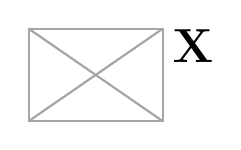
\begin{tikzpicture}
\draw[thstroke, draw=black!35] (0.000,0.000) -- (1.700,0.000);
\draw[thstroke, draw=black!35] (1.700,0.000) -- (1.700,1.172);
\draw[thstroke, draw=black!35] (1.700,1.172) -- (0.000,1.172);
\draw[thstroke, draw=black!35] (0.000,1.172) -- (0.000,0.000);
\draw[thstroke, draw=black!35] (0.000,0.000) -- (1.700,1.172);
\draw[thstroke, draw=black!35] (1.700,0.000) -- (0.000,1.172);
\node[anchor=north west, font=\LARGE\bfseries, inner sep=0pt] at (1.820,1.172) {X};
\end{tikzpicture}\\[1pt]\parbox[t]{2.90cm}{\centering\footnotesize \textbf{cross out}}\end{tabular}\hfill
\begin{tabular}[b]{@{}c@{}}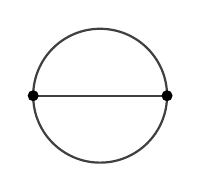
\begin{tikzpicture}
\draw[thstroke] (0.000,0.850) -- (1.700,0.850);
\draw[thstroke] (0.850,0.850) circle (0.850);
\fill (0.000,0.850) circle (0.07);
\fill (1.700,0.850) circle (0.07);
\end{tikzpicture}\\[1pt]\parbox[t]{2.90cm}{\centering\footnotesize start at a dot}\end{tabular}\hfill
\begin{tabular}[b]{@{}c@{}}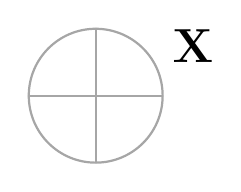
\begin{tikzpicture}
\draw[thstroke, draw=black!35] (0.000,0.850) -- (1.700,0.850);
\draw[thstroke, draw=black!35] (0.850,0.000) -- (0.850,1.700);
\draw[thstroke, draw=black!35] (0.850,0.850) circle (0.850);
\node[anchor=north west, font=\LARGE\bfseries, inner sep=0pt] at (1.820,1.700) {X};
\end{tikzpicture}\\[1pt]\parbox[t]{2.90cm}{\centering\footnotesize \textbf{cross out}}\end{tabular}\hfill
\begin{tabular}[b]{@{}c@{}}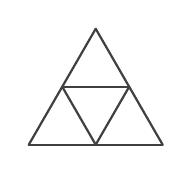
\begin{tikzpicture}
\draw[thstroke] (0.000,0.000) -- (1.700,0.000);
\draw[thstroke] (1.700,0.000) -- (0.850,1.472);
\draw[thstroke] (0.850,1.472) -- (0.000,0.000);
\draw[thstroke] (0.850,0.000) -- (1.275,0.736);
\draw[thstroke] (1.275,0.736) -- (0.425,0.736);
\draw[thstroke] (0.425,0.736) -- (0.850,0.000);
\end{tikzpicture}\\[1pt]\parbox[t]{2.90cm}{\centering\footnotesize start anywhere}\end{tabular}\hfill\null\par\smallskip

Cross out the envelope (rectangle with an X) and the circle with a plus. Why: a point where 3 lines meet has to be where you start or where you stop. Those two pictures have four such points, and you only get two.
\hints{1. ``Try the second copy, starting at a different corner.'' \;2. ``Start at a corner where 3 lines meet.'' \;3. House: ``Start at a bottom corner.''}

\kprob{Problem 6}{pages 9--10}{Draw one more bridge in each town so that you can pick up every counter.}
\par\smallskip\noindent\hfill\begin{tabular}[b]{@{}c@{}}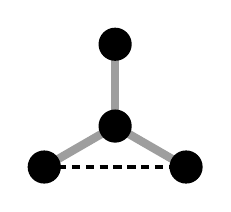
\begin{tikzpicture}
\draw[thband] (1.100,0.720) -- (1.100,1.759);
\draw[thband] (1.100,0.720) -- (0.200,0.200);
\draw[thband] (1.100,0.720) -- (2.001,0.200);
\draw[thnew] (0.200,0.200) -- (2.001,0.200);
\draw[thfill] (1.100,0.720) circle (0.200);
\draw[thfill] (1.100,1.759) circle (0.200);
\draw[thfill] (0.200,0.200) circle (0.200);
\draw[thfill] (2.001,0.200) circle (0.200);
\end{tikzpicture}\\[1pt]\parbox[t]{2.90cm}{\centering\footnotesize join two filled islands}\end{tabular}\hfill
\begin{tabular}[b]{@{}c@{}}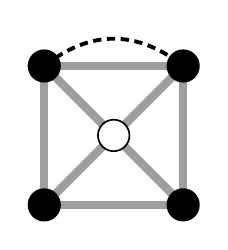
\begin{tikzpicture}
\draw[thband] (0.200,0.200) -- (1.964,0.200);
\draw[thband] (1.964,0.200) -- (1.964,1.964);
\draw[thband] (1.964,1.964) -- (0.200,1.964);
\draw[thband] (0.200,1.964) -- (0.200,0.200);
\draw[thband] (1.082,1.082) -- (0.200,0.200);
\draw[thband] (1.082,1.082) -- (1.964,0.200);
\draw[thband] (1.082,1.082) -- (1.964,1.964);
\draw[thband] (1.082,1.082) -- (0.200,1.964);
\draw[thnew] (0.200,1.964) .. controls (0.788,2.426) and (1.376,2.426) .. (1.964,1.964);
\draw[thfill] (0.200,0.200) circle (0.200);
\draw[thfill] (1.964,0.200) circle (0.200);
\draw[thfill] (1.964,1.964) circle (0.200);
\draw[thfill] (0.200,1.964) circle (0.200);
\draw[thisland] (1.082,1.082) circle (0.200);
\end{tikzpicture}\\[1pt]\parbox[t]{2.90cm}{\centering\footnotesize join two filled islands}\end{tabular}\hfill
\begin{tabular}[b]{@{}c@{}}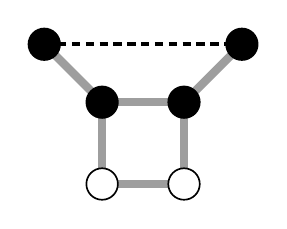
\begin{tikzpicture}
\draw[thband] (0.935,0.200) -- (1.975,0.200);
\draw[thband] (1.975,0.200) -- (1.975,1.239);
\draw[thband] (1.975,1.239) -- (0.935,1.239);
\draw[thband] (0.935,1.239) -- (0.935,0.200);
\draw[thband] (0.935,1.239) -- (0.200,1.975);
\draw[thband] (1.975,1.239) -- (2.710,1.975);
\draw[thnew] (0.200,1.975) -- (2.710,1.975);
\draw[thisland] (0.935,0.200) circle (0.200);
\draw[thisland] (1.975,0.200) circle (0.200);
\draw[thfill] (1.975,1.239) circle (0.200);
\draw[thfill] (0.935,1.239) circle (0.200);
\draw[thfill] (0.200,1.975) circle (0.200);
\draw[thfill] (2.710,1.975) circle (0.200);
\end{tikzpicture}\\[1pt]\parbox[t]{3.01cm}{\centering\footnotesize join two filled islands}\end{tabular}\hfill\null\par\smallskip

Each town has four islands with an odd number of bridges (filled). A new bridge joining any two of them works: six choices per town. The dashed line is one. A new bridge may run beside an old one. Afterwards, start on one of the two filled islands you did not join.
\hints{1. ``Where do you always get stuck? Try a new bridge from there.'' \;2. ``Which islands have 1 bridge or 3 bridges?'' \;3. ``Join two of those.''}

\kprob{Problem 7}{page 10}{Build two towns from 4 hexagons and craft sticks, one where the partner can pick up every counter and one where they cannot, and draw both.}
Answers vary. Can: a row of 4 hexagons (3 sticks), or a square (4 sticks). Cannot: one hexagon in the middle with a stick to each of the other three (the three-arm star from Problem 3). To check any town: count the sticks at each hexagon. It works only when no hexagon or exactly two hexagons have an odd number of sticks.
\hints{1. ``Build a town from Problem 3 that got an X.'' \;2. ``Make an island with only one bridge. Make another.''}

\kprob{Problem 8}{pages 11--12}{Put two counters on one bridge (so it can be crossed twice) and try to pick up every counter. Colour each bridge where that works.}
\par\smallskip\noindent\hfill\begin{tabular}[b]{@{}c@{}}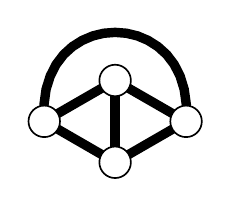
\begin{tikzpicture}
\draw[thbold] (1.100,1.239) -- (1.100,0.200);
\draw[thbold] (1.100,1.239) -- (0.200,0.720);
\draw[thbold] (1.100,1.239) -- (2.001,0.720);
\draw[thbold] (1.100,0.200) -- (0.200,0.720);
\draw[thbold] (1.100,0.200) -- (2.001,0.720);
\draw[thbold] (0.200,0.720) -- (0.197,0.935) -- (0.223,1.127) -- (0.276,1.296) -- (0.351,1.443) -- (0.446,1.568) -- (0.557,1.669) -- (0.682,1.748) -- (0.816,1.805) -- (0.956,1.839) -- (1.100,1.850) -- (1.244,1.839) -- (1.385,1.805) -- (1.519,1.748) -- (1.643,1.669) -- (1.755,1.568) -- (1.850,1.443) -- (1.925,1.296) -- (1.977,1.127) -- (2.004,0.935) -- (2.001,0.720) -- (2.001,0.720);
\draw[thisland] (1.100,1.239) circle (0.200);
\draw[thisland] (1.100,0.200) circle (0.200);
\draw[thisland] (0.200,0.720) circle (0.200);
\draw[thisland] (2.001,0.720) circle (0.200);
\end{tikzpicture}\\[1pt]\parbox[t]{2.90cm}{\centering\footnotesize all 6 bridges}\end{tabular}\hfill
\begin{tabular}[b]{@{}c@{}}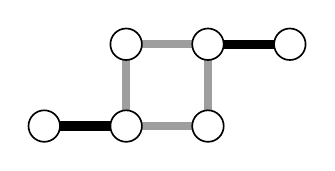
\begin{tikzpicture}
\draw[thband] (1.240,0.200) -- (2.279,0.200);
\draw[thband] (2.279,0.200) -- (2.279,1.239);
\draw[thband] (2.279,1.239) -- (1.240,1.239);
\draw[thband] (1.240,1.239) -- (1.240,0.200);
\draw[thbold] (0.200,0.200) -- (1.240,0.200);
\draw[thbold] (2.279,1.239) -- (3.319,1.239);
\draw[thisland] (1.240,0.200) circle (0.200);
\draw[thisland] (2.279,0.200) circle (0.200);
\draw[thisland] (2.279,1.239) circle (0.200);
\draw[thisland] (1.240,1.239) circle (0.200);
\draw[thisland] (0.200,0.200) circle (0.200);
\draw[thisland] (3.319,1.239) circle (0.200);
\end{tikzpicture}\\[1pt]\parbox[t]{3.62cm}{\centering\footnotesize only the 2 thick bridges}\end{tabular}\hfill
\begin{tabular}[b]{@{}c@{}}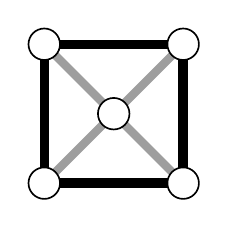
\begin{tikzpicture}
\draw[thbold] (0.200,0.200) -- (1.964,0.200);
\draw[thbold] (1.964,0.200) -- (1.964,1.964);
\draw[thbold] (1.964,1.964) -- (0.200,1.964);
\draw[thbold] (0.200,1.964) -- (0.200,0.200);
\draw[thband] (1.082,1.082) -- (0.200,0.200);
\draw[thband] (1.082,1.082) -- (1.964,0.200);
\draw[thband] (1.082,1.082) -- (1.964,1.964);
\draw[thband] (1.082,1.082) -- (0.200,1.964);
\draw[thisland] (0.200,0.200) circle (0.200);
\draw[thisland] (1.964,0.200) circle (0.200);
\draw[thisland] (1.964,1.964) circle (0.200);
\draw[thisland] (0.200,1.964) circle (0.200);
\draw[thisland] (1.082,1.082) circle (0.200);
\end{tikzpicture}\\[1pt]\parbox[t]{2.90cm}{\centering\footnotesize only the 4 thick bridges}\end{tabular}\hfill\null\par\smallskip

Arc town: all 6 bridges. Square with two tails: only the 2 tail bridges. Square with a centre island: only the 4 sides, not the 4 bridges to the centre.
\hints{1. ``Try one bridge, then another. Colour the ones that worked.'' \;2. ``Try a bridge between two islands that each have 3 bridges, or 1.''}

\subsection{Grades 2--3 (mathematician)}

\textbf{Core:} Problems 1--4. \textbf{Then} 5 and 6 (the rule). \textbf{Further:} 7--10. \textbf{If a child is struggling:} do Problem 1, then Problem 3 by walking (drop ``without walking''), then Problem 7; skip Problem 2. ``Odd island'' below means an island with an odd number of bridges.

{\small
\begin{xltabular}{\linewidth}{@{}L{1.45cm}YL{5.9cm}@{}}
\hline
\textbf{Problem} & \textbf{Answer} & \textbf{Hints, in order} \\ \hline
\endhead
1, p.\,1, core & House: from B or C, ending at the other, e.g.\ B A C B D E C. Triangle with tail: from A or C, e.g.\ A C B D C. Two double bridges: from any island, back to the start, e.g.\ A B C B A. & 1. ``Which counters are left when you get stuck?'' 2. ``Try another start.'' 3. ``Start at B'' (house) or ``at A'' (tail). \\ \hline
2, pp.\,2--3, core & Town 1: none (D has 5 bridges, A, C and F have 1). Town 2: start A or D, end at the other. Town 3: start D or F, end at the other. Town 4: any island, ending where it started. & 1. ``Keep a list: each island, did a walk from it work?'' 2. ``Write how many bridges each island has.'' 3. ``Compare the two lists.'' \\ \hline
3, pp.\,4--5, core & Big triangle: circle all six. Triangle with a double bridge: A and C. Arc town: none (all four odd). Square with three spokes: none (B, C, D, E odd). & 1. ``What did the starts in Problems 1 and 2 have in common?'' 2. ``Count the bridges at each island.'' 3. ``Look at the islands with an odd count.'' \\ \hline
4, pp.\,6--7, core & Each town has four odd islands: star A, B, C, D; square with tails B, C, D, E; ladder B, C, F, G. A new bridge joining any two of them works (6 per town); the walk then runs between the other two. Examples: star, add C--D: A B C D B. Tails, add B--E: C B E A B F E D. Ladder, add B--G: C B G C D H G F E A B F. & 1. ``Which islands do you get stuck on?'' 2. ``What does a new bridge do to the counts at its two ends?'' 3. ``Join two islands with odd counts.'' \\ \hline
5, pp.\,7--8 & House: 1 (a second B--C bridge, the only way). Arc town: 2 (A--B and C--D, or A--C and B--D, or A--D and B--C). H town: 3, pairing up all six islands, e.g.\ A--D, B--E, C--F (15 ways). Fewer cannot work: a new bridge changes the counts at only two islands. & 1. ``Which islands have odd counts?'' 2. ``How many of them can one new bridge fix?'' \\ \hline
6, p.\,8 & Count bridges at each island. All even: start anywhere, end where you started. Exactly two odd: start at one, end at the other. More odd: no walk. Child's reason: ``Each time you go through an island you come in on one bridge and leave on another, so you pick up its counters two at a time. An odd island has one left over, so you must start or finish there.'' & 1. ``Look back at your lists in Problems 2 and 3.'' 2. ``Did you ever see a town with exactly one odd island?'' 3. ``When you go through an island, how many of its counters do you take?'' \\ \hline
7, pp.\,8--9 & House yes (start at a bottom corner). Window no (the middles of the 4 sides have 3 lines). Star in pentagon yes, from anywhere. Envelope no (4 corners with 3 lines). Rings yes, from anywhere (8 crossings, 4 lines each). Square with diamond yes. Explanation: ``A point where 3 lines meet must be the start or the end. This picture has 4 of them.'' & 1. ``Try the second copy from a different point.'' 2. ``Count the lines at each corner and crossing.'' \\ \hline
8, p.\,10 & All four can be built; children must letter their hexagons. Checked examples: (1) A, B, C, D in a row with every bridge doubled; a double bridge is needed (with single bridges, 6 bridges on 4 islands join every pair once and every island is odd). (2) Triangle A B C with tails A--D and B--E. (3) Ring A B C D E F A plus A--C and C--F. (4) A--B once, A--C twice, B--C twice; any other way needs 3 sticks between one pair. & 1. ``Which islands must have an odd number of sticks?'' 2. ``Start from a town you know and change it one stick at a time.'' \\ \hline
9, p.\,11 & It cannot be done. If a walk from X ends at another island Y, walk it backwards: it starts at Y. If it ends back at X, start at the second island of the same walk and go round: another start. & 1. ``Take any walk. Can you walk it backwards?'' 2. ``And if it ends where it started?'' \\ \hline
10, p.\,12 & Arc town: 2, on two bridges with no island in common (A--B and C--D, A--C and B--D, or A--D and B--C). Three-arm star: 3, all three bridges, because each tip has only one bridge and needs an even count. & 1. ``Which islands have odd counts?'' 2. ``A second counter adds one crossing at both ends of its bridge.'' \\ \hline
\end{xltabular}
}

\subsection{Grades 4--5 (organizer)}

\textbf{Core:} Problems 1--5. \textbf{Further:} 6--11. \textbf{If a child is struggling:} Problems 1 and 3, then 5 with counters on the map's bridges; skip 2. Problems 1 and 2 are the same towns as 2--3 Problems 1 and 2.

{\small
\begin{xltabular}{\linewidth}{@{}L{1.45cm}YL{5.9cm}@{}}
\hline
\textbf{Problem} & \textbf{Answer} & \textbf{Hints, in order} \\ \hline
\endhead
1, p.\,1, core & House B to C, e.g.\ B A C B D E C. Tail town A to C, e.g.\ A C B D C. Doubles: anywhere, closed, e.g.\ A B C B A. & 1. ``Which counters are left?'' 2. ``Try another start.'' \\ \hline
2, pp.\,2--3, core & Town 1 none (D 5; A, C, F 1). Town 2: A and D. Town 3: D and F. Town 4: every island, closed. & 1. ``List starts that worked; write each island's bridge count.'' 2. ``Compare.'' \\ \hline
3, pp.\,4--5, core & 2 by 4 ladder: none (B, C, F, G have 3). Bowtie: anywhere, ending where it started. 3 by 3 grid with B--D: F to H or H to F only. & 1. ``What do the starts in Problem 2 have in common?'' 2. ``Count bridges at each island.'' \\ \hline
4, p.\,5, core & 0 odd islands: any start, closed. 2 odd: start at one, end at the other. More: none. Why: a walk takes the counters at an island it passes through in pairs (in, out); only the first and last island can have one unpaired. & 1. ``Look at the counts at islands where walks start and end.'' 2. ``Passing through an island, how many of its bridges do you use?'' \\ \hline
5, p.\,6, core & Bridges as drawn: A--B twice, A--C twice, A--D, B--D, C--D; counts A 5, B 3, C 3, D 3. No walk: four odd areas. One new bridge between any two areas works, and the walk then runs between the other two (B--C can cross the river west of A). Closed walk: 2 new bridges pairing the four areas (A--B with C--D, A--C with B--D, or A--D with B--C). Euler's own argument: a walk over 7 bridges names 8 areas in order; A (5 bridges) must appear 3 times and B, C, D twice each, which is 9. & 1. ``Count the bridges at each area.'' 2. ``Which part of your rule does this town break?'' 3. ``Which counts does a new B--C bridge change?'' \\ \hline
6, p.\,7 & No and no. Adding up the bridge counts of all islands counts every bridge twice (once at each end), so the total is even; an odd number of odd islands would make it odd. & 1. ``Add up the counts in a few towns. What do you get?'' 2. ``What does one bridge add to the total?'' \\ \hline
7, pp.\,7--8 & House 1 stroke (from a bottom corner). Window 2. Cube 4 (8 corners with 3 lines; the 2 crossings have 4). 3 by 3 grid 4 (8 edge points with 3 lines). Rings 1. Star 1. Fewest strokes is half the number of odd points: each stroke has two ends and each odd point is an end. & 1. ``Count lines at each point.'' 2. ``Where can a stroke start or stop?'' \\ \hline
8, p.\,9 & A B J I B C J E C D E F J H F G H I A. The inside bridges form three triangles through J: B I J, C E J, F H J. Go round one each time Lee's walk reaches B, C and F. 352 walks work (keeping Lee's direction on each bridge). & 1. ``Which bridges are left after Lee's walk?'' 2. ``Where do those touch Lee's walk?'' 3. ``At B, go round B J I and back to B.'' \\ \hline
9, p.\,10 & All even: start anywhere and walk until stuck; you can only be stuck back at the start, because any other island has an unused bridge each time you arrive. If counters remain, some island on your loop still has one (the town is connected); walk a new loop from there and splice it in. Repeat. Two odd islands: add a bridge between them, take the closed walk, then remove that bridge from it. & 1. ``Walk until you are stuck. Where can that happen?'' 2. ``Counters are left: start a new loop from an island you passed.'' 3. ``For two odd islands, add one bridge.'' \\ \hline
10, pp.\,11--12 & Numbers are (route that ends where it started, route that may end anywhere). Arc town (2, 1): two bridges with no island in common; open: any one bridge. Three-arm star (3, 1): all three bridges; open: any one. Diagonals town (2, 0): D--E and E--F, or D--B and B--F; open needs none, since only D and F are odd. & 1. ``Which islands are odd?'' 2. ``What does an extra counter do to the counts at the ends of its bridge?'' \\ \hline
11, p.\,12 & All four islands are odd. A closed route needs every count even, and each extra counter changes the counts at the two ends of its bridge only, so it fixes at most two islands. At least 2 are needed, and 2 work. & 1. ``How many islands must change?'' 2. ``How many can one extra counter change?'' \\ \hline
\end{xltabular}
}

\section{The mathematics behind the week}

\textbf{Euler's theorem.} A connected multigraph has a trail through every edge exactly once if and only if it has 0 or 2 vertices of odd degree. With 0, every such trail is closed and can start anywhere; with 2, every such trail runs from one to the other. \emph{Necessity:} each interior visit to a vertex uses two of its edges, so only the two ends of the trail can have odd degree (and none, if the trail is closed). \emph{Sufficiency} (Hierholzer, 1873): if all degrees are even, walk from $v$ until stuck; you can only be stuck at $v$, since arriving at $w\ne v$ has used an odd number of $w$'s edges. If edges remain, connectivity gives a vertex $u$ on the circuit with an unused edge; the unused edges still have all degrees even, so a closed trail from $u$ in them exists and is spliced in at $u$. With two odd vertices $a,b$, add an edge $ab$, take an Euler circuit and delete the edge.

\textbf{Handshake lemma.} $\sum_v \deg v = 2|E|$, so the number of odd vertices is even (4--5 Problem 6). The set of possible start vertices is therefore all vertices, two vertices, or empty, never one (2--3 Problem 9). One new edge between two odd vertices removes both from the odd set (K--1 Problem 6, 2--3 Problem 4); with $2k$ odd vertices a closed walk needs exactly $k$ new edges if they may join any pair (2--3 Problem 5).

\textbf{Königsberg} has degrees 5, 3, 3, 3. Euler (1736) did not draw a graph; he counted letters: a walk over 7 bridges is a sequence of 8 land areas, and an area with $k$ bridges ($k$ odd) appears $(k+1)/2$ times, giving $3+2+2+2=9>8$.

\textbf{One-stroke drawings.} Take corners, ends and crossings as vertices. A connected drawing with $2k>0$ odd points needs exactly $k$ strokes (Listing, 1847): each stroke has two ends and every odd point is an end of some stroke; conversely, add $k-1$ edges pairing odd points, take an Euler trail, and cut it at the added edges.

\textbf{Delivery routes} (Chinese postman problem: Kwan Mei-Ko 1962; Edmonds and Johnson 1973). The repeated crossings form an edge multiset $J$ such that every vertex has even degree in $G+J$; each repeated edge flips the parity of its two ends, so $J$ is a union of paths pairing up the odd vertices. The minimum is a minimum-weight perfect matching of the odd vertices under shortest-path distance; for an open route, leave the best pair unmatched. The bound ``half the number of odd vertices'' (4--5 Problem 11) is not always reached: the three-arm star has 4 odd vertices but needs 3 (paths of length 1 and 2).

\textbf{Where it goes next.} Directed graphs: an Euler circuit exists if and only if in-degree equals out-degree everywhere; this gives de Bruijn sequences (the shortest cyclic string containing every $n$-bit word). The BEST theorem counts Euler circuits. Fleury's algorithm is the counters' own advice: never cross a bridge that cuts you off from counters you still need, unless there is no other choice. The contrast worth showing 4--5: visiting every island exactly once (a Hamiltonian path) has no parity rule and no known fast test.

Sources: Euler, \emph{Solutio problematis ad geometriam situs pertinentis} (1736); Biggs, Lloyd and Wilson, \emph{Graph Theory 1736--1936}, ch.\,1; Levin, \emph{Discrete Mathematics: An Open Introduction}, \S4.4; Edmonds and Johnson (1973).

\clearpage
\section{What to write down after the session}

Each adult fills in this page for their table, the same evening if possible. Photograph any town a child built or drew (K--1 Problem 7, 2--3 Problems 8 and 9) and any page with a claim written on it.

Claims to listen for. \textbf{K--1:} ``Start on an island with 3 bridges.'' ``A tip with one bridge is a dead end.'' ``We tried every island, so it can't be done.'' \textbf{2--3:} ``The walk starts and ends at the odd islands.'' ``There is never just one odd island.'' \textbf{4--5:} ``The number of odd islands is always even.'' ``Extra counters needed = half the number of odd islands'' (false: the three-arm star in Problem 10 needs 3).

\begin{tabularx}{\linewidth}{@{}L{3.3cm}Y@{}}
\hline
Problems reached & Circle per child or pair: K--1 \,1 2 3 4 5 6 7 8\quad 2--3 \,1 \dots\ 10\quad 4--5 \,1 \dots\ 11 \\
What they tried & e.g.\ tried every island in turn; counted bridges; started from tips; rebuilt a town with sticks to test a rule. \\
What they said & Children's words, quoted. \\
Drawing or claim to keep & One per table, e.g.\ a town a child designed, or a sentence such as ``start where there are three bridges''. \\ \hline
\end{tabularx}

For each claim, tick how far it got, and sketch one drawing worth keeping:

\begin{tabularx}{\linewidth}{@{}YL{1.3cm}L{1.3cm}L{2.2cm}L{1.6cm}@{}}
\hline
Claim, in the child's words & tried & guessed & checked in some cases & explained \\ \hline
\rule{0pt}{18pt} & & & & \\ \hline
\rule{0pt}{18pt} & & & & \\ \hline
\rule{0pt}{18pt} & & & & \\ \hline
\rule{0pt}{18pt} & & & & \\ \hline
\end{tabularx}

\medskip
\noindent\begin{tikzpicture}\draw[black!60] (0,0) rectangle (\linewidth-1pt,5.5cm); \node[anchor=north west, font=\footnotesize] at (0.1,5.4) {Drawing (a town or picture a child made, with who made it):};\end{tikzpicture}

\end{document}
